% Ramanujan tau(n) for n = 1..12, from q * prod (1-q^n)^24. Positive bars charcoal, negative bars coral.
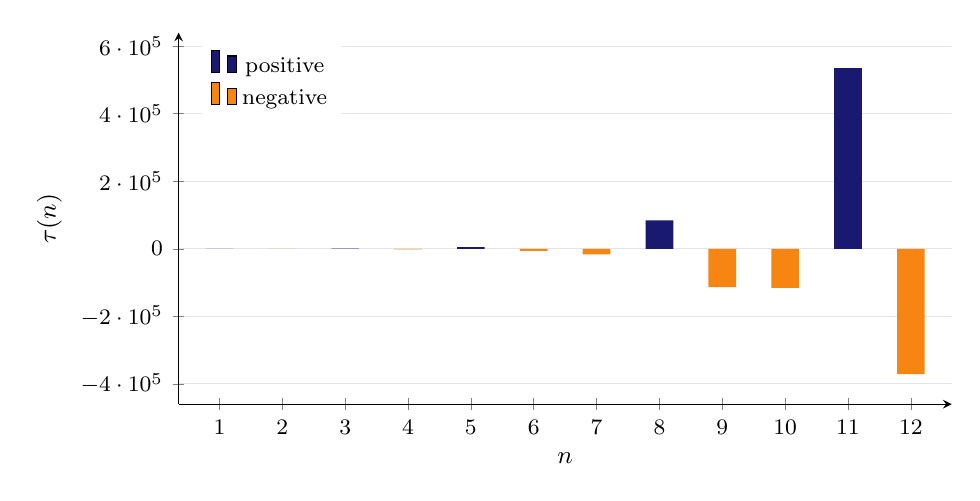
\begin{tikzpicture}
\begin{axis}[
  width=11.4cm,
  height=6.3cm,
  ybar,
  bar width=10pt,
  xmin=0.35,
  xmax=12.65,
  ymin=-460000,
  ymax=640000,
  xtick={1,2,3,4,5,6,7,8,9,10,11,12},
  xlabel={$n$},
  ylabel={$\tau(n)$},
  axis lines=left,
  ymajorgrids,
  grid style={MidnightBlue!12},
  tick label style={font=\footnotesize},
  label style={font=\small},
  legend style={font=\footnotesize, at={(0.03,0.97)}, anchor=north west, draw=none},
  scaled y ticks=false,
  ytick={-400000,-200000,0,200000,400000,600000}
]
\addplot[ybar, bar shift=0pt, fill=MidnightBlue, draw=none] coordinates {
  (1,1)
  (3,252)
  (5,4830)
  (8,84480)
  (11,534612)
};
\addlegendentry{positive}
\addplot[ybar, bar shift=0pt, fill=BurntOrange, draw=none] coordinates {
  (2,-24)
  (4,-1472)
  (6,-6048)
  (7,-16744)
  (9,-113643)
  (10,-115920)
  (12,-370944)
};
\addlegendentry{negative}
\end{axis}
\end{tikzpicture}
